\documentclass[conference]{IEEEtran}
\usepackage[T1]{fontenc}
\usepackage{graphicx,amsmath,amssymb,booktabs,url}
\usepackage[hidelinks]{hyperref}
\graphicspath{{images/}}
\title{Inventory Image Tagging, Phase 2: A Small CNN, an Ablation Study and a CNN--Classifier Hybrid}
\author{\IEEEauthorblockN{Aryan, Divyanshu Singh, Jatin Kumar Singh, Jatin Verma, Kushagra Bhardwaj}
\IEEEauthorblockA{Enrolments: 2401020013, 2401010161, 2401010199, 2401010200, 2401010247\\
Section B. Contact: aryan.kinha2024@nst.rishihood.edu.in}}
\begin{document}
\maketitle
\begin{abstract}
Phase 1 classified Fashion-MNIST clothing pictures with fixed descriptions (pixels, HOG) and classical classifiers; its best model, Pixels with Random Forest, reached 87.61\% test accuracy and confused shirts, T-shirts, pullovers and coats. We train a small convolutional neural network (CNN) on the same 48,000 training pictures, choose every setting on the same 12,000 validation pictures, and score the official 10,000 test pictures once. An ablation study with three seeds per setting tests batch normalisation, dropout, augmentation and depth. We also test a hybrid that gives the CNN's 64 learned features to a Phase 1 classifier. The CNN reaches $91.98\pm0.24$\% test accuracy and the hybrid $92.49\pm0.19$\%. Shirt recall rises from 59.2\% to 73.6\% (CNN) and 75.7\% (hybrid). Most ablation differences are close to the seed-to-seed spread, and dropout of 0.4 reduced accuracy.
\end{abstract}
\begin{IEEEkeywords}Fashion-MNIST, convolutional neural network, ablation, regularisation, hybrid model\end{IEEEkeywords}

\section{Introduction}
Phase 1 described each $28\times28$ picture by a fixed list of numbers chosen before any model saw the data. Flattened pixels keep every brightness value but not which pixels are neighbours; HOG summarises local edge directions but fixes the description in advance. Its best model confused upper-body categories: only 59.2\% of shirts were found.

A CNN learns its own description. Small shared filters measure local patterns, pooling keeps the strongest responses, and later layers combine them. We ask three questions. Does a small CNN beat the Phase 1 models on the same protocol? Which of its ingredients matter? Does a classical classifier on the CNN's learned features improve on the CNN's own last layer? The code, saved predictions and checkpoints are in the project repository.

\section{Related Work}
LeCun et al.~\cite{lecun} introduced convolution, weight sharing and pooling for document recognition. Krizhevsky et al.~\cite{alexnet} showed that ReLU units, dropout and augmentation let a deep CNN generalise on large images. Srivastava et al.~\cite{dropout} describe dropout; Ioffe and Szegedy~\cite{bn} describe batch normalisation and note it can also regularise. Kingma and Ba~\cite{adam} describe Adam. Prechelt~\cite{prechelt} compares early-stopping criteria. Simard et al.~\cite{simard} found that distorting training pictures slightly helps a CNN.

For the hybrid, Razavian et al.~\cite{razavian} fit a linear SVM on features from a pretrained CNN and obtained strong results; Tang~\cite{tang} replaced the softmax layer with a linear SVM trained jointly. We differ from both: our CNN is trained on this dataset only, and the classifier is fitted afterwards. Xiao et al.~\cite{fashion} introduced Fashion-MNIST. Reported gains from batch normalisation, dropout and augmentation on small CNNs are modest, so we measure them with several seeds instead of assuming them.

\section{Data and Protocol}
We reuse the Phase 1 split: official training pictures divided by a stratified split with seed 42 into 48,000 for training and 12,000 for validation, plus the official 10,000 test pictures. Pixels are divided by 255. All training, selection and early stopping use training and validation pictures only. The settings were written to \textit{reports/phase2/frozen.json} before the test pictures were scored, and a marker file blocks a second test run. Phase 1 predictions on the same test pictures give a paired comparison.

Every setting was trained with three seeds (42, 1, 2); we report the mean and sample standard deviation. Macro F1 is the mean of the ten per-category F1 scores, so every category counts equally.

\section{Architecture}
\begin{figure*}[t]\centering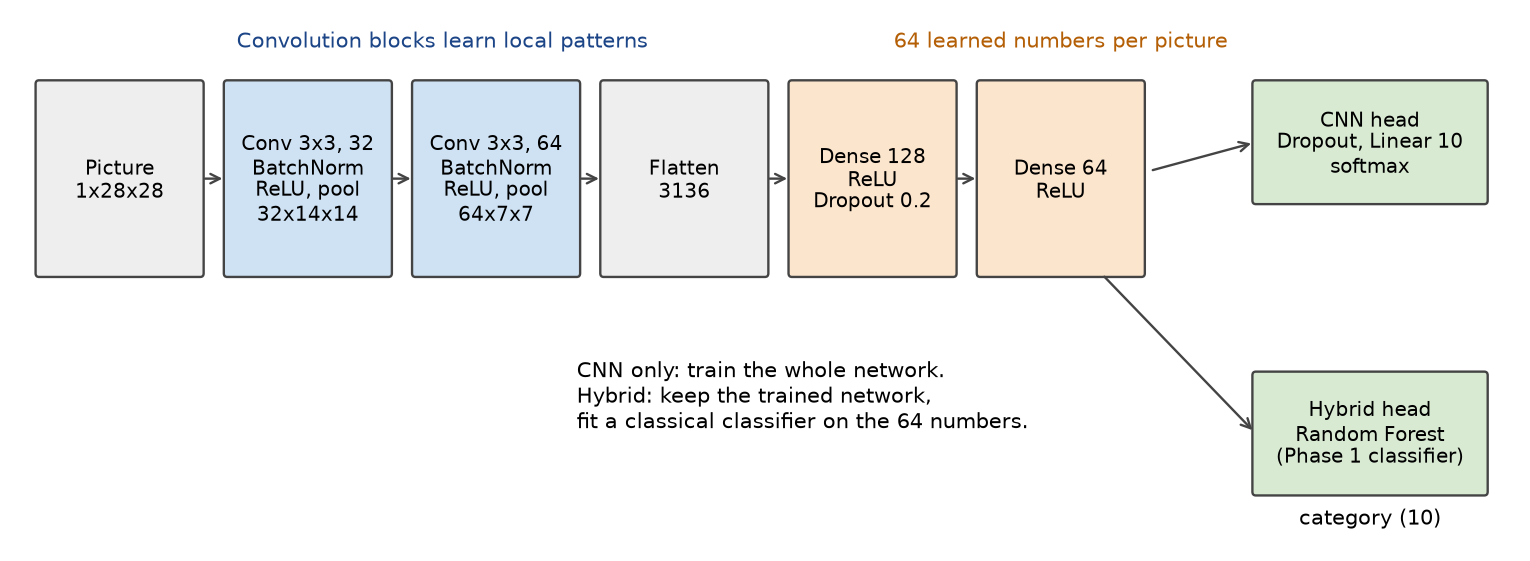
\includegraphics[width=\textwidth]{architecture.png}
\caption{The network and the two ways to finish. The 64 numbers after the dense layers are the learned features.}\label{fig:arch}\end{figure*}
Figure~\ref{fig:arch} shows the network. Each convolution block applies $3\times3$ filters, batch normalisation, ReLU and $2\times2$ max pooling:
\[h_{c}(i,j)=\max\!\Big(0,\ \sum_{u,v}w_{c}(u,v)\,x(i+u,j+v)+b_c\Big),\]
and pooling takes the maximum over each $2\times2$ patch, halving the width and height ($28\to14\to7$). Weight sharing means a filter needs 9 weights wherever the pattern appears. A $3\times3$ filter sees a small neighbourhood; after two blocks each unit depends on a larger part of the picture, which lets deeper blocks combine edges into shapes such as sleeves or collars.

The $64\times7\times7=3136$ values pass through dense layers of 128 and 64 units (ReLU, dropout between them) to a linear layer with ten outputs. The network has 429,450 trainable weights. We chose two blocks because pictures are only $28\times28$; after two poolings they are $7\times7$, and a third pooling would leave $3\times3$. The ablation tests a third block.

\section{Regularisation and Training}
\textbf{Batch normalisation} rescales each channel in a batch, $\hat{x}=(x-\mu_B)/\sqrt{\sigma_B^2+\epsilon}$, then applies a learned scale and shift. It uses batch statistics in training and stored averages in evaluation. \textbf{Dropout} sets each unit to zero with probability $p$ during training and rescales the rest by $1/(1-p)$; all units are used at test time. \textbf{Augmentation} mirrors each training picture left to right with probability $0.5$ and shifts it by up to two pixels in each direction, filling with black. A mirrored or nudged garment keeps its category. Test pictures are never altered. \textbf{Weight decay} of $10^{-4}$ shrinks weights slightly at every step.

The loss is cross-entropy, $-\frac1n\sum_i\log p_{y_i}(x_i)$, minimised with Adam~\cite{adam} (learning rate $10^{-3}$, batches of 128, at most 30 epochs). \textbf{Early stopping:} after each epoch we compute validation loss; training stops after five epochs without improvement, and the weights of the best epoch are restored. Reported scores never come from a later, more overfit epoch. Figure~\ref{fig:curves} shows the final model: training loss keeps falling while validation loss flattens.
\begin{figure}[t]\centering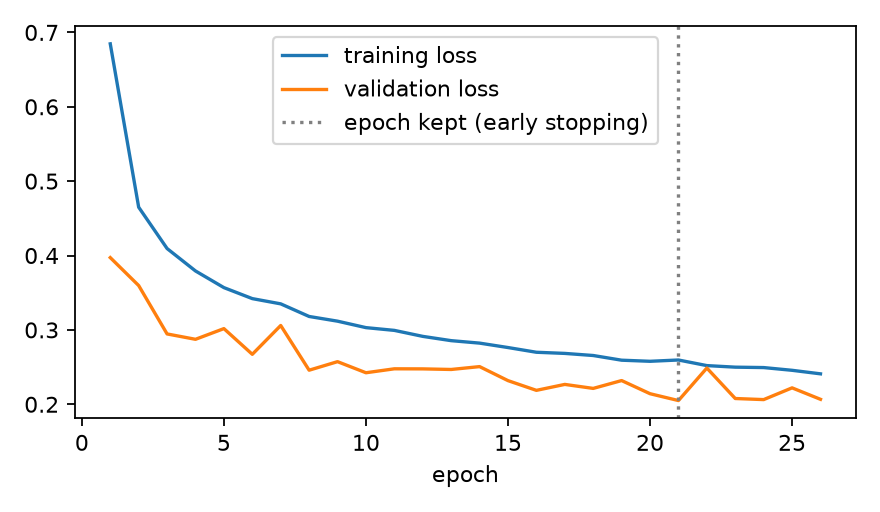
\includegraphics[width=0.9\columnwidth]{learning_curves.png}
\caption{Loss per epoch, final CNN, seed 42.}\label{fig:curves}\end{figure}

\section{Ablation Study}
We remove one ingredient at a time from a full model (batch normalisation, dropout 0.4, augmentation, two blocks), add a three-block version, and run a plain model with none of the three ingredients. Light dropout (0.2) was added after the first runs showed that 0.4 hurt; it was judged on validation data only. Table~\ref{tab:ablation} and Fig.~\ref{fig:ablation} give validation macro F1.
\begin{table}[t]\centering\caption{Ablation, validation macro F1 (mean $\pm$ std of 3 seeds).}\label{tab:ablation}
\begin{tabular}{lc}\toprule
Version & Macro F1\\\midrule
No dropout & $0.9282\pm0.0022$\\
Light dropout 0.2 (final) & $0.9264\pm0.0033$\\
Plain & $0.9258\pm0.0023$\\
No augmentation & $0.9254\pm0.0033$\\
Three blocks & $0.9215\pm0.0049$\\
Full (dropout 0.4) & $0.9202\pm0.0036$\\
No batch norm & $0.9195\pm0.0018$\\\bottomrule\end{tabular}\end{table}
\begin{figure}[t]\centering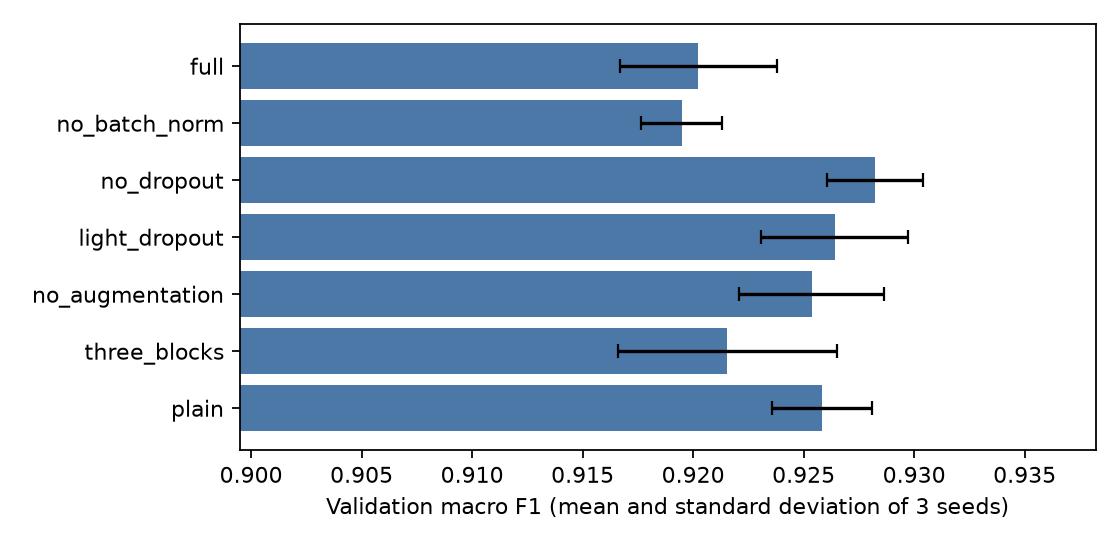
\includegraphics[width=\columnwidth]{ablation.png}
\caption{Ablation. Bars show the mean, whiskers one standard deviation.}\label{fig:ablation}\end{figure}

All seven versions lie within 0.9 points, and most gaps are about as large as the seed-to-seed spread, so we rank them loosely. Dropout of 0.4 reduced macro F1 by 0.8 points compared with no dropout; dropout of 0.2 is close to no dropout. Our reading is that at this size the network overfits little, so strong regularisation costs accuracy; we did not test this further. Augmentation and batch normalisation showed no clear gain here, and a third block did not help. The project brief asks for a CNN with dropout, so the final model is the best version that uses it (light dropout, 0.9264). The best version overall, no dropout, is 0.0018 higher, which is smaller than one standard deviation.

\section{Hybrid Approach}
The CNN's second dense layer gives a vector $z\in\mathbb{R}^{64}$ per picture. Instead of the final linear layer we fit a Phase 1 classifier on $z$ from the training pictures: Logistic Regression, linear SVM or Random Forest, each with the two Phase 1 settings, chosen by validation macro F1. The reason is that the final layer is one linear map, while a forest or a margin classifier may draw a better boundary around the same features. The classifier is fitted after the CNN is trained, not jointly.

Two checks keep the claim honest. First, the CNN's own last layer is the comparison. Second, a control uses features from an untrained CNN of the same shape. On validation data the selected Random Forest reaches macro F1 $0.9324$, against $0.9264$ for the CNN's last layer and $0.7944$ for the untrained-network control. The control shows that training, not only the architecture, makes the features useful. The three classifier families land within 0.15 points of each other, and even Logistic Regression gains about half a point, so the gain comes from refitting on the learned features rather than from the forest itself.

\section{Results}
Table~\ref{tab:test} gives test results. The CNN and the hybrid use three seeds each. A paired bootstrap over the 10,000 test pictures (2,000 resamples, seed 42 models) gives an accuracy difference of $+4.10$ points for the CNN over the Phase 1 best, 95\% interval $[+3.52,+4.67]$, and $+0.60$ points for the hybrid over the CNN, interval $[+0.28,+0.94]$. The three-seed means differ by 0.51 points.
\begin{table}[t]\centering\caption{Official test set, scored once.}\label{tab:test}
\begin{tabular}{lcc}\toprule
Model & Accuracy & Macro F1\\\midrule
Phase 1: Pixels + RF & 87.61\% & 0.8747\\
CNN (3 seeds) & $91.98\pm0.24$\% & $0.9194\pm0.0032$\\
Hybrid, CNN + RF (3 seeds) & $92.49\pm0.19$\% & $0.9246\pm0.0020$\\\bottomrule\end{tabular}\end{table}

\textbf{Similar categories.} Figure~\ref{fig:recall} and Table~\ref{tab:recall} compare recall. The CNN removes most Pullover--Coat confusion (116 to 33 pullovers called coats) and raises Shirt recall by 14 points, yet about one shirt in four is still wrong. Figure~\ref{fig:errors} shows pictures the CNN gets right and Phase 1 gets wrong, and pictures both get wrong; several of the latter are long-sleeved tops with unusual patterns or shapes. The pictures alone cannot show whether a label is wrong.
\begin{table}[t]\centering\caption{Test recall (CNN and hybrid: mean of 3 seeds).}\label{tab:recall}
\begin{tabular}{lccc}\toprule
Category & Phase 1 & CNN & Hybrid\\\midrule
T-shirt/top & 85.2 & 88.9 & 88.5\\
Pullover & 80.2 & 88.7 & 89.6\\
Coat & 82.2 & 87.0 & 88.2\\
Shirt & 59.2 & 73.6 & 75.7\\\bottomrule\end{tabular}\end{table}
\begin{figure}[t]\centering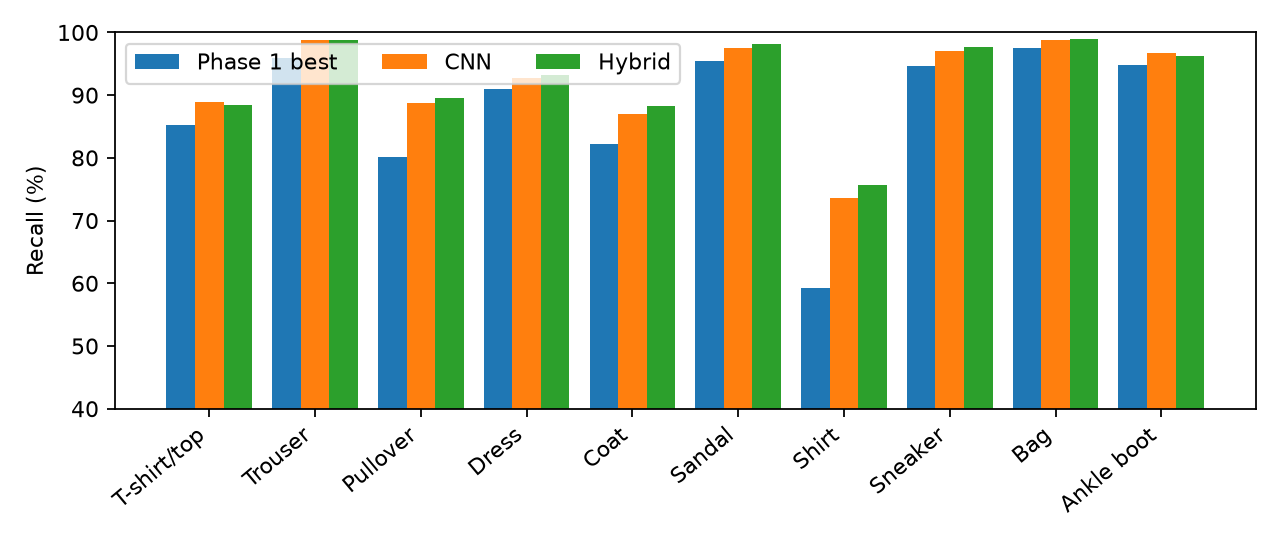
\includegraphics[width=\columnwidth]{recall_comparison.png}
\caption{Per-category test recall.}\label{fig:recall}\end{figure}
\begin{figure}[t]\centering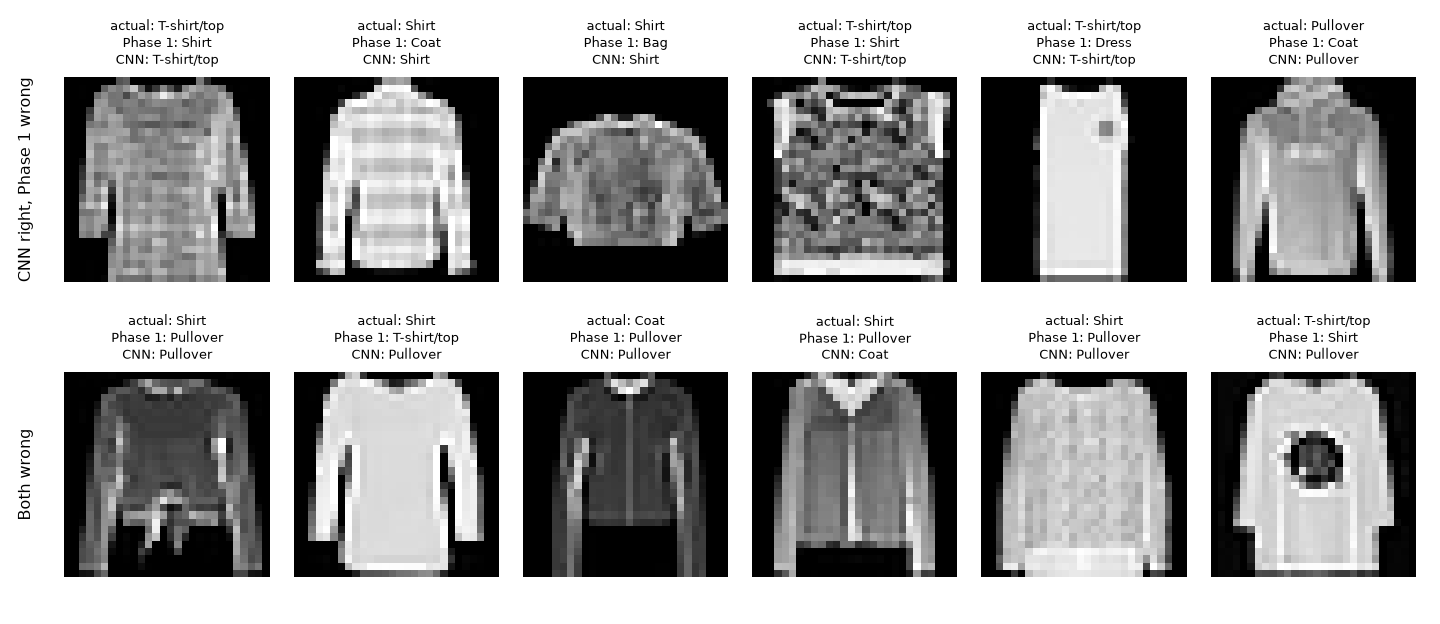
\includegraphics[width=\columnwidth]{error_examples.png}
\caption{Upper-body test pictures: CNN right and Phase 1 wrong (top); both wrong (bottom).}\label{fig:errors}\end{figure}

\textbf{Cost.} On the same CPU with two threads, from picture to label, the CNN takes 0.17\,ms per picture and 429,450 weights (1.7\,MB). The Phase 1 forest took 24.98\,ms (measured in an earlier session on the same machine). The hybrid takes 25.88\,ms because its 400-tree forest dominates.

\section{Technical Validation and Limitations}
Tests recompute every reported score from the saved predictions, check the committed checkpoints against the saved hashes, check that the frozen choices match the selection files, and check that the Phase 2 split equals Phase 1. A reload of the committed checkpoint reproduces the saved test predictions. Training on an Apple GPU is not exactly repeatable, so a rerun can differ slightly.

Limits: Fashion-MNIST is a small, centred, familiar benchmark, and these results say little about real catalogue photos. We use one split, three seeds and a small search. In the hybrid, the classifier is fitted on training-picture features from a network that already saw those pictures, which may make them look cleaner than features of new pictures. Light dropout and the rule ``best version that uses dropout'' were added after seeing validation results; the test pictures played no part in either. We did not test residual networks, pretrained models, schedules or other augmentations because they add machinery beyond the problem.

\section{Conclusion}
A two-block CNN with batch normalisation, light dropout, augmentation and early stopping beat the best Phase 1 model by about four points and helped most with Pullover, Coat and Shirt. Feeding its 64 learned features to a Random Forest added about half a point more. Most ablation choices mattered less than the seed-to-seed spread, and heavy dropout hurt. The CNN is not in the live dashboard.

\begin{thebibliography}{12}
\bibitem{lecun} Y. LeCun, L. Bottou, Y. Bengio, and P. Haffner, ``Gradient-based learning applied to document recognition,'' \emph{Proc. IEEE}, vol. 86, no. 11, pp. 2278--2324, 1998.
\bibitem{alexnet} A. Krizhevsky, I. Sutskever, and G. E. Hinton, ``ImageNet classification with deep convolutional neural networks,'' in \emph{Advances in Neural Information Processing Systems 25}, 2012.
\bibitem{dropout} N. Srivastava, G. Hinton, A. Krizhevsky, I. Sutskever, and R. Salakhutdinov, ``Dropout: a simple way to prevent neural networks from overfitting,'' \emph{J. Mach. Learn. Res.}, vol. 15, pp. 1929--1958, 2014.
\bibitem{bn} S. Ioffe and C. Szegedy, ``Batch normalization: accelerating deep network training by reducing internal covariate shift,'' in \emph{Proc. ICML}, 2015, arXiv:1502.03167.
\bibitem{adam} D. P. Kingma and J. Ba, ``Adam: a method for stochastic optimization,'' in \emph{Proc. ICLR}, 2015, arXiv:1412.6980.
\bibitem{prechelt} L. Prechelt, ``Early stopping---but when?'' in \emph{Neural Networks: Tricks of the Trade}, LNCS 1524, Springer, 1998.
\bibitem{simard} P. Y. Simard, D. Steinkraus, and J. C. Platt, ``Best practices for convolutional neural networks applied to visual document analysis,'' in \emph{Proc. ICDAR}, 2003, pp. 958--962.
\bibitem{razavian} A. S. Razavian, H. Azizpour, J. Sullivan, and S. Carlsson, ``CNN features off-the-shelf: an astounding baseline for recognition,'' in \emph{CVPR Workshops}, 2014, arXiv:1403.6382.
\bibitem{tang} Y. Tang, ``Deep learning using linear support vector machines,'' arXiv:1306.0239, 2013.
\bibitem{fashion} H. Xiao, K. Rasul, and R. Vollgraf, ``Fashion-MNIST: a novel image dataset for benchmarking machine learning algorithms,'' arXiv:1708.07747, 2017.
\end{thebibliography}
\end{document}
